\bibliography{SBC_Ausarbeitung_Dimitrijevic_Traxler}
\documentclass[a4paper,12pt]{scrreprt}
\usepackage[T1]{fontenc}
\usepackage[utf8]{inputenc}
\usepackage[ngerman]{babel}
\usepackage[table]{xcolor}% http://ctan.org/pkg/xcolor
\usepackage{tabu}
\usepackage{graphicx}
\usepackage{lmodern}

\begin{document}


%\titlehead{Kopf} %Optionale Kopfzeile
\author{Daniel Dimitrijevic \and Thomas Traxler} %Zwei Autoren
\title{ Space Based Computing } %Titel/Thema
\subject{VSDB} %Fach
\subtitle{ Ausarbeitung } %Genaueres Thema, Optional
\date{\today} %Datum
\publishers{5AHITT} %Klasse

\maketitle
\tableofcontents



\chapter{Erklärung}
	\section{Wofür steht Space-Based Computing?}
		Space-Based Computing (fortan SBC) hat seine Ursprünge im parallel programming, und stellt dabei hauptsächlich ein Datenorientiertes Modell zur Koordination und Kommunikation dar. Wie aus dem Namen eindeutig hervorgeht handelt es sich um ein Modell welches auf 'Spaces' basiert. Ein Space ist gleichbedeutend mit einem (logischen) Ort auf welchem Daten von mehreren Komponenten geteilt verwendet werden. Diese Komponenten können im einfachsten Fall 'write', 'read' und 'take' Aktionen ausführen. Ein Write steht dabei für das zur Verfügung Stellen eines neuen Datenteils an alle anderen Komponenten in diesem Space, ein Read für das Lesen von Daten ohne diese zu entfernen und ein Take für das Lesen und Entfernen einer Datei aus dem Space, auch destructive-read genannt. Im einfachsten Fall hat ein Space nun das Datenmodell eines Tuples.\\ Eine Hauptanforderung die an einen Space  gestellt wird ist das persistente Aufbewahren aller Daten die sich in ihm befinden, auch bei Systemausfällen. Wie das SBC modelliert und implementiert wird kann sehr stark variieren, je denn gegebenen Anforderungen und Wünschen entsprechend. Was hierbei vor allem variiert ist die Zahl der Geräte auf dem der Space implementiert ist und die Zahl der Geräte die auf diesen Space zugreifen, diese Zahlen sind prinzipiell, wenn nicht durch den Anwendungsfall anders umgesetzt, voneinander unabhängig und befinden sich jeweils im Bereich von 1 bis n. \\   Das SBC-System stellt eine logische zentrale Einheit dar, welche nicht spezifiziert wo genau sie Physikalisch vorhanden ist. Der Ort, an dem eine Datei schlussendlich abgespeichert wird, kann dabei nach verschiedensten Methoden ausgewählt werden. In der simpelsten Form wird das selbe Prinzip wie bei Tuples angewendet %TODO Nachschaun
		oder es werden Prinzipien  wie FIFO, LIFO, keys, geo-coordinates verwendet wahlweise auch noch kompliziertere, auch das ist vom gegebenen Anwendungsfall abhängig.
		%\cite{Steinmetz2005} 
		%TODO Zitieren
		\subsection{EAI}
			Enterprise Application Integration (EAI) Systeme sind der heutige Ansatz um der oft allgemein üblichen 'chaotischen' Kommunikation entgegen zu wirken. Gemeint sind damit beispielsweise Sockets, MOM, RPC oder RMI die meistens nur so wie es gerade notwendig ist direkt mit allen Möglichen anderen Komponenten kommunizieren, zwar genau so wie es für ihre Aufgabe notwendig ist im Gesamtbild aller Komponenten jedoch eben Chaotisch. \\
			EAI Systeme sind Beispielsweise Object Request Broker (CORBA DCOM...), Message Queues, Message Broker und Enterbrise service Buses.\\
			All diese Systeme sind jedoch hauptsächlich Nachrichten-orientiert und ziemlich komplex, daher für Kommunikation zwar brauchbar, jedoch für tatsächliches Arbeiten mit verteilt abgespeicherten Daten nur bedingt ratsam, an dieser Stelle kommt nun SBC ins Spiel.
		
		\subsection{Unterschied zwischen SBC und Cloudcomputing}
			Um nun der Verwechslung von SBC und Cloudcomputing vorzubeugen sei nun gesagt, zu aller erst behandelt SBC lediglich die Daten und Cloudcomputing stellt noch viele weitere Ressourcen (wie zB. Rechenleistung) zur Verfügung. Auch zu Cloud-Storrage kann man abgrenzen, Cloud-Storrage behandelt nicht nur die interne Abspeicherung der Daten sondern auch vor allem wie diese dem Benutzer zur Verfügung gestellt und abstrahiert werden, bei SBC geht es hauptsächlich um die interene Verteilung und Kommunikation der Komponenten untereinander und stellt dabei einen Datenkanal zwischen den Komponenten des Spaces dar beziehungsweise zur Verfügung. 
			
	\section{Einsatzbereiche}
		SBC wird vor allem immer dort verwendet wo Daten verteilt abgespeichert werden sollen. Dies kann auf verschiedenste Arte durchgeführt werden um so 'Bottlenecks' %TODO Fußnote
		zu schließen. SBC bietet durch die Verteilung des Spaces auf mehrere Komponenten grundlegend immer mehr zur Verfügung stehenden Speicherplatz, wodurch man je nach Implementierung verschiedene Vorteile gewinnen kann. Man kann diesen Speicherplatz beispielsweise direkt logisch zur Verfügung stellen und so den zur Verfügung stehenden Speicherplatz erhöhen, man kann die notwendige  Kommunikation auf einer Komponente verringern (durch Aufteilung) und man kann für Redundanz sorgen. Die Vorteile lassen sich auch annähernd beliebig kombinieren, wobei zu beachten ist, dass 2 kombinierte Vorteile auch bei bester Umsetzung, so gut wie immer einen dritten Vorteil verringern oder noch andere Nachteile mit sich ziehen. Redundanz schlägt sich Beispielsweise immer auf den zur Verfügung stehenden Speicherplatz nieder, was durch erhöhte Kommunikation zwischen den Komponenten jedoch wieder verringert werden kann. \\    Ein Beispiel für einen weiteren Vorteil wäre zum Beispiel die Möglichkeit an jeder Komponente Zugang zum ganzen Space zu haben, was in einem Master-Client System erhöhte Kommunikation zum Master mit sich bringt, außerdem müssen die Clients in diesem Fall auch durchgehend die Möglichkeit haben zumindest einen Master ansprechen zu können. Dieser Vorteil stellt sich automatisch ein wenn man auf ein Peer-to-Peer System wechselt, wobei auch oftmals stark belastete Master-Komponenten nicht mehr notwendig sind aber in der Regel wieder mehr Kommunikation zwischen den Komponenten notwendig ist.
\chapter{Grundlegende Prinzipien}
	
	\section{Space-Based Computing Paradigma}
		Interaktionen sind bei SBC in 3 Teile geteilt 
		\begin{itemize}
			\item Zeit
				\subitem Applikationen können jederzeit Daten lesen und schreiben.
			\item Space
				\subitem Applikationen müssen nur auf den selben Space zugreifen um miteinander zu kommunizieren
			\item Referenzierung
				\subitem Applikation die miteinander Kommunizieren müssen nicht tatsächlich voneinander wissen.
		\end{itemize}
		Durch diese Aufteilung sind die Applikation tatsächlich voneinander unabhängig, ändert sich nun an einer Applikation etwas (Ort, Ausführungszeit etc.) so ist dies für die andere gänzlich irrelevant (abgesehen von sich ändernden Inhalt) solange sich der Space auf den beide zugreifen und über welchen sie Kommunizieren der gleiche bleibt. Auch wenn zu einem späteren Zeitpunkt weitere Applikation hinzugefügt werden, so ist das (erneut, ausgenommen Nachrichteninhalt) für die ersten beiden Applikation insofern irrelevant als das man an ihnen nichts ändern muss deswegen. Zu beachten ist jedoch dass so keine direkte Kommunikation mehr stattfindet und daher auch keine direkte Reaktion zu erwarten ist in der Regel. (Ausgenommen es werden Notifies ausgeschickt)
		
		
		
	\section{Mapping}
		Mapping ist ein sehr essentieller Teil des SBC, hierbei wird definiert wie eine Applikation tatsächlich von ihrer Anfrage an den Space, zu den abgespeicherten Daten bzw. zu dem Ergebnis der Anfrage kommt. Dafür ist in jedem Fall ein einheitliches Konzept für den gesamten Space, bzw. für das ganze Space-System notwendig. Nach diesem Konzept wird auf den Space zugegriffen und anfragen gegebenenfalls Umgewandelt (zB. ein SBC read zu einem SQL select), außerdem ist in diesem Konzept auch eindeutig fest zu legen in welcher Form Daten schlussendlich im Space abgelegt sein können. (Datenbank, Plaintext, Bytestream, diverse Strukturtypen, etc.) \\
		Dieses Mapping hängt folglich stark von der Art des implementierten Systems ab, stellt ein Peer-to-Peer System beispielsweise gänzlich andere Anforderungen an einen Zugriffsvorgang als eine Server-Client Architektur und auch bei dieser kann es sich sehr unterscheiden ob es nur ein Server ist oder bei Replikation, auf die Art der Replikation. Der nutzen von gutem Mapping kann beginnen bei einheitlichen Daten die ohne sehr viel weiteres Marshalling meist auskommen bis hin zu Load Balancing, erhöhter Ausfallsicherheit, verringerte Zugriffszeiten/schnellere Anfragenabarbeitung, Ablaufoptimierung und mehr.
	
\chapter{Im Genaueren betrachtet}
	\section{Tuple Spaces}
		
		Ein Tupel Raum ist eine Ausführung des assoziativen Gedächtnissmodelles für verteiltes / parallele Verarbeitung. Es bietet eine Bibliothek von Tupeln, auf  die gleichzeitig zugegriffen werden kann. Tupel sind Mengen, mit null oder mehr Argumente und einem Schlüssel. \\		
		Die Sammlung von Tupeln unterstützt einige Grundfunktionen, wie zB das Hinzufügen eines Tupels in den Raum (Schreiben) und Entfernen eines Tupels aus dem Raum (nehmen). Das Tupel Sammlung wird von einem Netzwerk über mehrere Server aufbewahrt und gemanaged. Mehrere Threads können zur selben Zeit auf den selben Raum zugreifen.
		
		\subsection{Linda}
		Ziel von Linda ist es, Prozessen einer Anwendung zu erlauben, miteinander zu kommunizieren, ohne Informationen zur Identifikation des Datensatzes zu wissen. Linda geht von einem Tupelraum  als Umgebung aus. Verschiedene nebenläufige Prozesse eines verteilten Programms kommunizieren über einen gemeinsamen Tupelraum dadurch, dass jeder dieser Prozesse diesem Tupelraum beliebig Tupel hinzufügen und Tupel daraus entfernen kann.\\\\	
		Die daraus resultierende zeitliche und räumliche Entkoppelung ermöglicht einen Entwurf verteilter Protokolle, die flexibel und robust auf die Herausforderungen verteilter Programmierung reagieren können wie z.B auf Latenz, erhöhten Synchronisationsaufwand und mögliche Teilausfälle des Systems. 
		
		
		\section{Triple Spaces}
		
		Bis jetzt werden die meisten "Messages" direkt zwischen den Maschinen ausgetauscht. Triple Space Computing möchte das die Daten in einen
		Space geschrieben werden und das jeder auf die Elemente des Spaces zugreifen kann und diese lesen/schreiben/entnehmen kann.\\ %TODO Zitat
		'In der Zukunft könnte Triple space Computing das Web für die Maschine werden wie HTML das Web für Menschen geworden ist'\lbrack Zitat: http://www.tripcom.org/\rbrack.\\ \\
		Triple Space Computing bietet ein Kommunikationsparadigma für anonymen und asynchronen Informationsaustausch und ebenfalls die Persistenz und einzigartige Identifikation von Daten.\\
			
		

\begin{figure}[h]
\centering
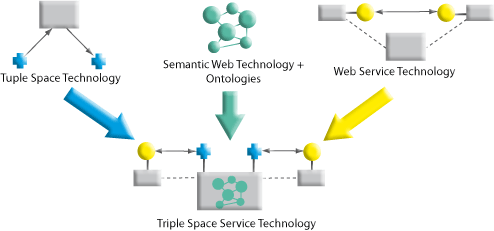
\includegraphics[width=0.7\linewidth]{./tripcom_overview2}
\caption{}
\label{fig:tripcom_overview2}
\end{figure}
\lbrack Quelle: http://tripcom.org/,19.12.2013\rbrack

\begin{figure}[h]
\centering
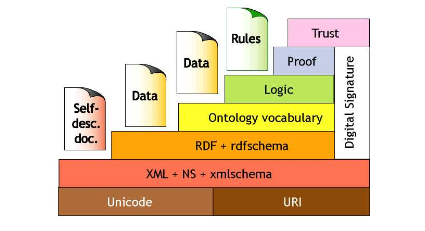
\includegraphics[width=0.7\linewidth]{./Semantic_Web_www_tripcom_org_docs_coordination07_paper}
\caption{}
\label{fig:Semantic_Web_www_tripcom_org_docs_coordination07_paper}
\end{figure} %TODO Caption einfügen
\lbrack Quelle: www.tripcom.org/docs/coordination07/paper\rbrack \\\\\\ 

		
		
	
		
			Die Semantische Web Technologie ist eine Erweiterung des heutigen Webs, in dem die Informationen eine gut definierte, maschinell verarbeitbare Bedeutung haben und es Maschinen und Menschen ermöglicht leicht zu Co-Operieren.\\
				Es ist gedacht um das Web mit einem Netzwerk von adressierbaren URIs zu verlinken so ,dass es Maschinen leicht fällt syntaktisch und semantisch darauf zuzugreifen.
				Für diesen Zweck sollten die Ressourcen mit Maschinen verständlichen Metadaten versehen werden, die durch Verwendung von Allgemeinem Vokabular und einer vordefinierten Semantik erreicht werden, auch bekannt als "Ontologie"
				\\
			
	

		
			
		
		
		%TODO Muss ich mir nochmal web services anschauen. Referenzieren auf SOA ausarbeitung
		Die Web-Service Technologie bietet eine 
		"Virtuelle Komponenten-Modell" zur Vereinfachung der 
		heterogenen Welt von Komponenten. Es  erlaubt es, bestehende Funktionalität zu nutzen 
		ohne die Last der Middleware spezifischen Eigenheiten, wie die invokation-Mechanismus, Transport-Protokoll usw. Web Services sind eine gut verstandene Kommunikationsstruktur und-Architektur für Unternehmensanwendungen.\\ Mehr zu diesem Thema in der Ausarbeitung über SOA.
		
		\section{Reliable Message}
			
			Reliable Message verhält sich wie Tuple Space computing. Nur, dass man hier nicht von Tuples spricht sondern von Messages.  Die Reliable Message Technologie geht von mehreren Channels aus die die geteilte Daten beinhalten und jeder dieser Channel kann von einem oder mehreren Server „unterstützt“ werden d.H. die geteilten Daten liegen auf einem oder mehreren Servern und können damit abgesichert werden. 
		
		\section{Peer-to-Peer Architekturen}
			
			Peer-to-Peer (fortan p2p) Architekturen bieten nun ganz eigene Möglichkeiten aber auch Anforderungen an und für ein SBC System. P2p bedeutet Gleichheit aller Komponenten, mindestens insofern, als dass es keine bestimmenden und steuernden (Master) Komponenten gibt, alle Komponenten gleichgestellt sind. Wobei zu beachten ist, dass es nicht nur erlaubt, sonder erwünscht ist, wenn Unterschiede bezüglich zB. den Komponenten zur Verfügung stehenden Ressourcen berücksichtigt werden. 
			
			\subsection{Weshalb p2p bei SBC?}
				
				Ein (gutes) p2p System bietet vor allem die Möglichkeit einfach Komponenten hinzu zu fügen, heraus zu nehmen oder aus zu tauschen, was gerade für einen Space der nicht vollständig definiert sein muss einen guten Vorteil bieten kann. Durch eine p2p Lösung kann sehr oft hohe Flexibilität des Systems erreicht werden, es sei nun gleich angemerkt, sollten die Anforderungen möglichst effiziente Nutzung von begrenzten oder klar definierten Ressourcen sein, so ist dies zu berücksichtigen und ein p2p Ansatz sehr wahrscheinlich nicht die beste Lösung. \\
				Ein p2p System liefert einem außerdem den Vorteil, dass man bei sehr dynamischen Systemen nicht oder nur bedingt darauf achten muss, dass alle Komponenten Arten (zB. Master-Servant) in einem effizienten Gleichgewicht zueinander stehen da Prinzipiell alle Komponenten der selben Art entsprechen sollten.
				
			\subsection{P2p Arten/Routing}
			
				Die Arten von p2p Systemen kann man in der Regel dadurch unterscheiden wie das Routing innerhalb des Systems funktioniert, d.h. wie schafft es Komponente A mit Komponente B-Z Kontakt auf zu nehmen. Das Routing in (größeren) p2p Systemen ist entscheidend dafür wie skalierbar, effizient, sicher und ressourcenschonend es ist.
				\\\\Prinzipiell kann man p2p Systeme in Unstrukturierte und Strukturierte Systeme unterteilen. Unstrukturierte Systeme stellen dabei den weit bekannteren Teil der Systeme und umfassen unter anderem zentralisierte Systeme (zB. Napster), Pure p2p Systeme (zB. Gnutella 0.4) oder Hybride p2p Systeme (zB. Gnutela 0.6) wärend Strukturierte p2p Systeme beispielsweise mit Distributed-Hash-Tables realisiert werden können. %\footnote{\cite{Steinmetz2005}}
				
			\subsection{Unstrukturierte p2p Systeme}
				\subsubsection{Zentralisiertes p2p}
					
					Zentralisiertes p2p ist nur bedingt ein tatsächliches p2p System. Es besteht zwar durchaus aus vielen gleichberechtigten Komponenten (zb. Datenspeichereinheiten) welche die Kommunikation und Organisation selbstständig regeln, jedoch existiert dabei ein zentraler Server bei welchem sich die Peers registrieren müssen und welcher den Peers die Information mitteilt wie diese den von ihnen gesuchten Peer erreichen können. Dies führt zwar einerseits zu geringerem Traffic zwischen den Peers da diese lediglich mit der zentralen Einheit kommunizieren müssen um einen anderen Peer zu erreichen, außerdem müssen die Peers lediglich abspeichern wie sie den zentralen Server erreichen, jedoch entspricht es nur bedingt tatsächlich dem p2p Konzept.\\
					Die Sicherheit des Systems hängt direkt von der der Sicherheit der Zentralen Einheit ab.
					
				\subsubsection{Pures p2p}
					
					Ein pures p2p System besteht aus x gleichberechtigten Komponenten die eine Verbindung mit y (y<x) Komponenten besitzen. Hier existiert keine zentrale Einheit und jede Komponente versucht möglichst direkt Kontakt mit jeder anderen Einheit auf zu nehmen. Wie das Routing innerhalb des Systems durchgeführt wird kann sehr unterschiedlich sein, jedoch ist es in der Regel bis zu einem gewissen Grad 'chaotisch', da es auf sehr kurzfristige Änderungen reagieren können muss. Pures p2p ist in der Regel sehr dynamisch da jederzeit neue Komponenten an jedem Ort hinzu kommen können und diese Verbindungen zu allen Möglichen anderen Komponenten ziehen können, bzw. permanent abspeichern wie diese erreichbar sind. Da dies jedoch meist (pseudo-)zufällig vonstatten geht ist Effizienz sehr oft nicht gegeben da zB. geographische Verteilung oder Belastbarkeit der Knoten nicht berücksichtigt wird. Das hingegen kann dazu führen dass man eine Komponente erreichen will die im Nebenraum platziert ist aber aufgrund des chaotischen Routings und der chaotischen Verbindungsfindung dafür über 3 Kontinente geroutet wird.
					
				\subsubsection{Hybrid p2p}
				
					Hybrid p2p ist eine Kombination aus zentralisiertem und purem p2p. Bei hybridem p2p bilden die Komponenten des Systems 'Gruppen' nach bestimmten Faktoren (meistens geographische Verteilung) und bestimmen eine oder mehrere Hauptkomponenten welche den Großteil des Routings zu den anderen Gruppen übernimmt. Die bestimmte Hauptkomponente ist in der Regel die welche am meisten Netzwerklast verarbeiten kann und am meisten Kontaktdaten zu anderen Komponenten abspeichern muss. Diese lokale Hauptkomponente ist dadurch in der Ausübung ihrer eigentlichen Tätigkeit eingeschränkt, jedoch erhält das gesamte Netzwerk so eine Struktur welche den Nachteilen der chaotischen Verbindungsführung entgegenwirkt und es kann dennoch leicht dynamisch gehalten werden da bei Ausfall einer Hauptkomponente einfach eine neue bestimmt werden kann. Auch kann man Gruppen wieder zu Gruppen zusammenfassen. (zB. Gruppenebene 1 fasst alle Komponenten eines Landes zusammen, Gruppenebene fasst alle Gruppen der ersten Ebene eines Kontinents zusammen)\\
					Hybrid p2p Systeme werden auch als 2. Generation unstrukturierter p2p Systeme bezeichnet.
					
			\subsection{Distributed Hash Tables}
				
				Distributed Hast Tables (fortan DHT) stellen den angeführten Vertreter von strukturierten p2p Systemen dar. Bei einem strukturierten System ist zu jederzeit eine ganz bestimmte Komponente für eine (bzw. mehrere) ganz bestimmte Anfrage zuständig. und zwar insofern als dass für jede theoretisch mögliche Anfrage innerhalb des Systems eine Komponente zuständig ist, nicht mehr und nicht weniger. \\Um diesen recht abstrakten Satz nun ein wenig zu veranschaulichen, nehmen wir an ziel des Systems ist es eine Datenbank auf zu bauen. So hat jeder Datensatz einen eindeutigen ihm zugehörenden Hashwert, für diesen Hashwert ist nun eine spezielle Komponente zuständig und diese muss wissen wo dieser Datensatz genau zu finden ist. \\ Ein konkreteres Beispiel: Die Datensätze bekommen einen Hashwert im Bereich 1 bis 9 und wir haben 3 Komponenten. Jede Komponente ist nun für einen Bereich der Hashwerte zuständig, sprich Komponente 1 muss wissen wo sich datensätze 1 bis 3 befinden und welche Komponente sie benachrichtigen kann um Datensätze 4-9 zu finden. Wie vorallem das finden der Datensätze 4-9 Implementiert ist und wie aufgeteilt wird welche Komponente für welchen Hashwert zuständig ist hängt vom verwendeten DHT-Algorithmus ab. Um das vorherige Beispiel ein wenig praxisnäher zu bringen könnte man den Hashwert 1 ersetzen durch alle MD5 Haswerte die mit 1 beginnen oder ähnliches.
				\pagebreak
				\subsubsection{Chord Algorithmus}
					\begin{figure}[h]
						\centering
						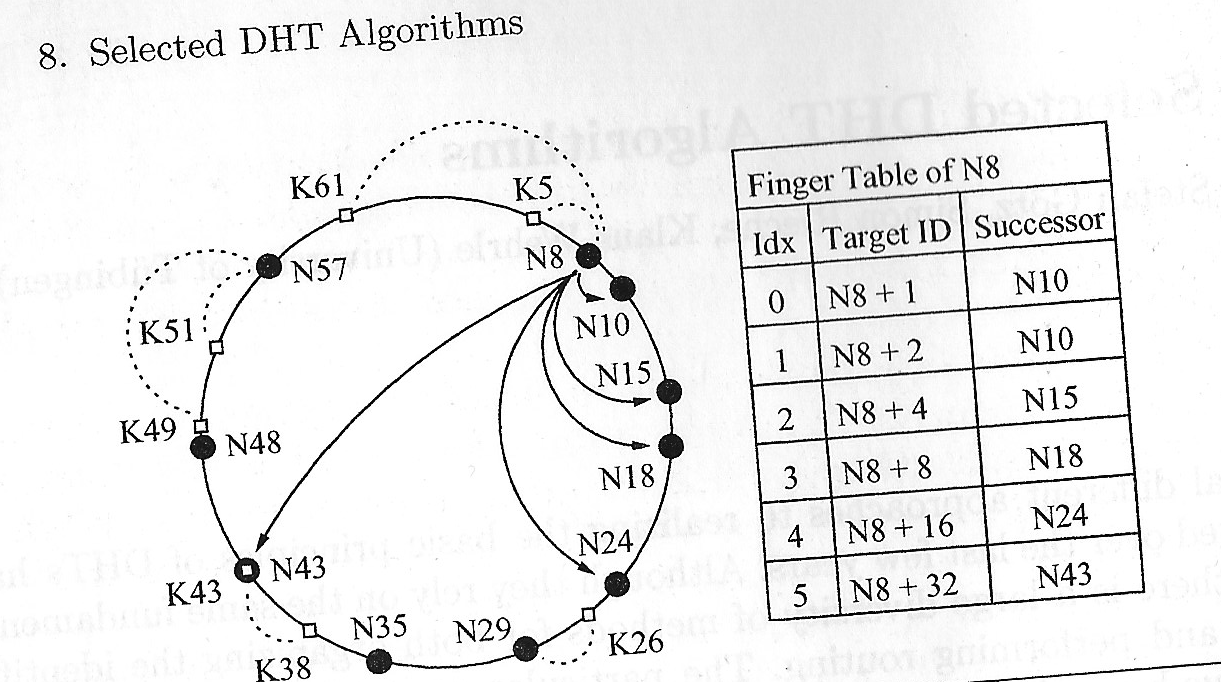
\includegraphics[width=0.7\linewidth]{./graphics/Chord}
						\caption{6-Bit Chord identifier Space. Gepunktete Linien geben an welche Komponenten (Nodes) welchen Key zu den Datensätzen betreuen.}
						\label{fig:Chord}
					\end{figure}

					Der Chord Algorithmus legt alle möglichen Hashwerte in einem Kreis ab. Jede Komponente muss nun wissen wo sie die Datensätze findet für die sie selbst zuständig ist (Für N8 Beispielsweiße K58-K8) und eine gewisse Anzahl anderer Komponenten nach folgendem Schema:\\
					'Each node maintains a routing table, the finger table, poiting to other nodes on the identifier circle. Given a circle with l-bit identfiers, a finger table has a maximum of l entries. On node n, the table entry at row i identifies the first node that succeeds n by at least $2^{i-1}$, i.e., successor $n+{2}^{i-1}$, where $1 <= i <= l$. For example, the second finder of node N8 $(8+2^1=10)$ is node 10 and the third finder $(8+2^2=12)$ is node 15' Wobei zu beachten ist,dass N15 für den Bereich der Keys 11 bis 15 zuständig ist. %TODO Zitieren.
					\\Dadurch ergeben sich selbst bei großen Speicher-Spaces (zB. 256 Bit) relativ kleine Finger Tables nur und somit auch nur kleiner Speicheraufwand zum Routing und erreichen aller Datensätze. Das Routing selbst wird immer genauer je näher man dem gewünschten Key kommt, die Anzahl der Routing-schritte befindet nicht daher im Bereich von O(log(N)). \\
					Würde N8 in unserem Beispiel (Abb.:\ref{fig:Chord}) K38 erreichen wollen so würde er den näherstehen vorhergehenden Node im Figure Table fragen, d.h. N24. N24 würde das selbe nun wieder machen, daher die Anfrage zu N35 weiterschicken. Bei N35 ist der näherste Node zu K38 ident mit dem ersten Node im Figur Table (N43), N35 würde N8 daher nun eine Nachricht schicken dass N43 für K38 zuständig ist. Würde N8 dagegen K51 wissen wollen wären die Schritte N43-N48 und dieser würde dann N57 als Antwort schicken.\\
					In einem Chord Netzwerk mit 1000 Komponenenten werden ungefähr O(10) Schritte gebraucht um die zuständige Komponente für den gesuchten Key zu finden. Der Chord Algorithmus hat außerdem die Möglichkeit zur Selbstorganisation bei neu hinzukommenenden Komponenten und Komponentenausfall
					%TODO Reference Steinmetz Seite 97
					
					
				\subsubsection{CAN Algorithmus}
					\begin{figure}[h]
						\centering
						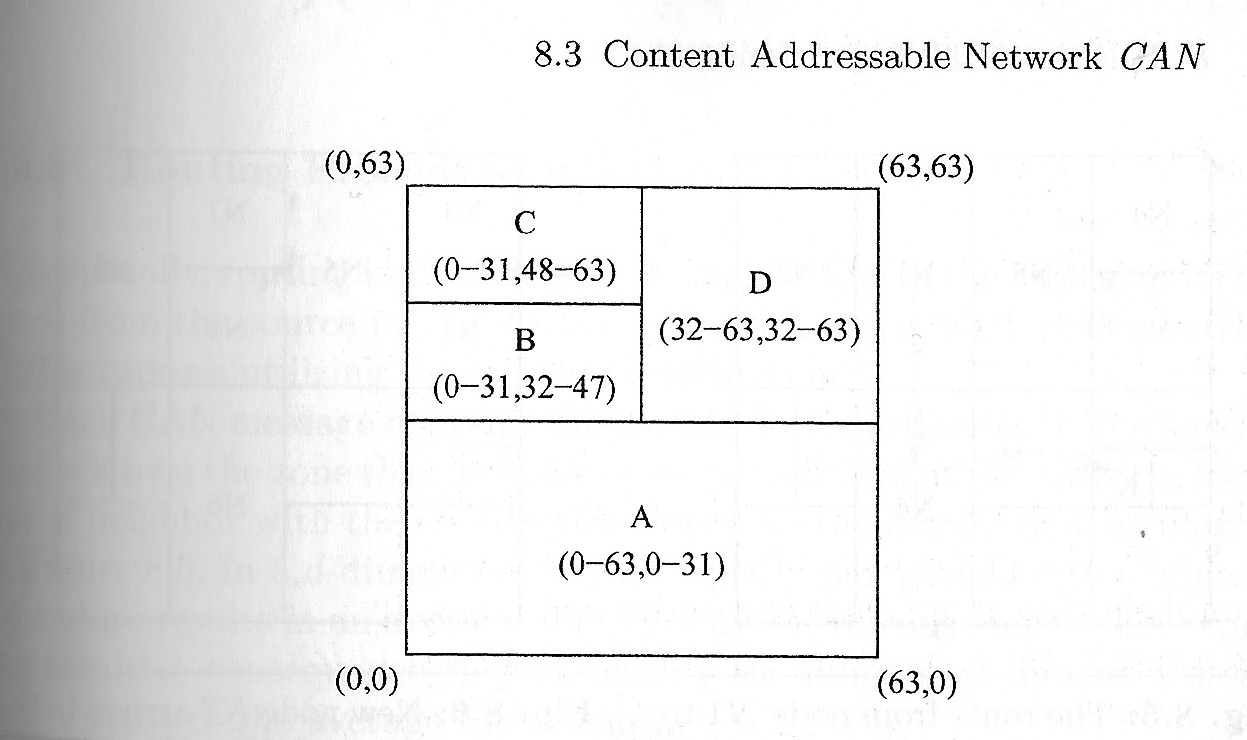
\includegraphics[width=0.7\linewidth]{./graphics/CAN}
						\caption{}
						\label{fig:CAN}
					\end{figure}
					Der CAN Algorithmus ist der zweite in dieser Ausarbeitung vorgestellte Algorithmus für DHT bzw. strukturiertes p2p. Er ist dem Chord Algorithmus sehr ähnlich hat jedoch zwei sehr große Unterschiede. Der Erste ist, dass jede Komponente nur mit ihrem direkten Nachbarn kommuniziert wenn ein bestimmtes Element gesucht ist (durch die Strukturierung ist die Richtung bekannt), der zweite Unterschied ist die Lösung aus der eindimensionalen Kante eines Kreises hin zur n-dimensionalen Identifizierung von Daten. \\
					In unserem Beispiel handelt es sich um einen zweidimensionalen 6-Bit Space der unter 4 Komponenten (A-D) aufgeteilt ist. Bei diesem System speichert jede Komponente ab welcher Nachbar für die gesuchte Koordinate zuständig ist. Außerdem werden die Dimensionen nacheinander durch gegangen.
					\\In Abbildung \ref{fig:CAN_Routing} wird beispielsweise die Y-Achse zuerst abgearbeitet. Allerdings ist es nicht zwingend notwendig das alle Komponenten die Dimensionen in der selben Reihenfolge abarbeiten. Das Routing in Abbildung \ref{fig:CAN_Routing} könnte genauso gut auch über N5 statt N6 stattfinden. Wird bei N1 wie abgebildet die Y-Achse zuerst abgearbeitet muss dieser nur folgende drei Einträge abspeichern um durch den gesamten Space routen zu können: N6 ist Zuständig für die gesamte x-Dimension wenn y kleiner N1, N2 ist für die gesamte x-Dimension größer N1 zuständig wenn y ident N1, N5 ist für die gesamte x-Dimension kleiner N1 zuständig wenn y ident N1.\\
					Die schlussendliche tatsächlich Effizienz des Algorithmus gegenüber anderen Algorithmen hängt sehr stark von dem Verhältnis der Anzahl der Komponenten zur Anzahl der Dimensionen ab. Die exakte Größenordnung für die Anzahl der Routingschritte und der Anzahl der notwendigen Nachrichten bei einer neuen Komponente ist O($(D/2)*N^{1/D}$), die Größenordnung für die Anzahl an notwendigen Einträgen zum Routing per Node und der notwendigen Nachrichten beim entfernen einer Komponente ist O(2*D).
					\begin{figure}
						\centering
						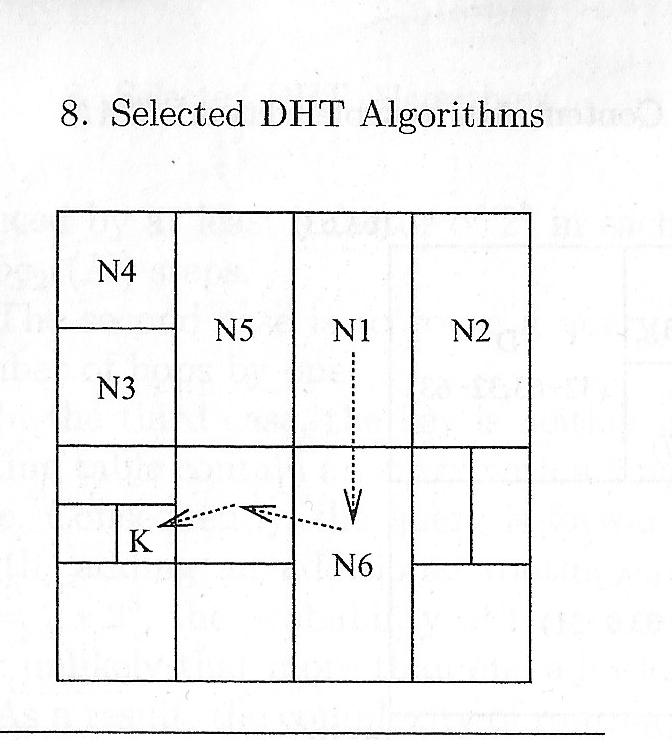
\includegraphics[width=0.55\linewidth]{./graphics/CAN_Routing}
						\caption{Routing in einem zweidimensionalen CAN-Space}
						\label{fig:CAN_Routing}
					\end{figure}
					 
\chapter{Namhafte Implementierungen}
	\section{JavaSpaces}
		JavaSpaces ist eine Spezifikation des Konzepts von Object-Spaces in der Programmiersprache Java. Ein Object-Space ist ein assoziativer Speicher von verteilten, über das Netz erreichbaren Objekten. Kommunikationspartner (peers) kommunizieren ausschließlich indirekt über diese Objekte. Dadurch etabliert der JavaSpace einen 'aktiven, verteilten Datenraum', wie er in keiner anderen Technologie geschaffen wird. Einige Ansätze der Jini-Technologie kommen hierbei zur Anwendung. Bei der Idee, die sich hinter den JavaSpaces verbirgt, handelt es sich nicht um eine revolutionäre Neuerung, sondern sie basiert im Wesentlichen auf den Linda TupelSpaces.\\\\	
		Die Gründe, warum JavaSpaces eingesetzt werden, sind vielfältig. Meist wird Skalierbarkeit und Verfügbarkeit bei gleichzeitiger Reduzierung der Gesamtkomplexität angestrebt.
		
		
		\section{Corso} %TODO bitte noch ein wenig besser Formatieren
			Corso( Co-ORdinated Shared Objects) basiert auf Forschungsarbeiten der Technischen Uni Wien.
			Software Entwicklung in heterogenen verteilten Systemen bringt immer zusätzlich Komplexität.\\\\
			•   Adressierung und Lokalisierung \\
			•	Replikation\\
			•	Transaktion\\
			•	Skalierbarkeit\\
			•	Lastverteilung\\
			•	Ausfallsicherheit\\ \\
			Corso ist eine Middleware die auf dem MOM(Message Oriented Middleware) Prinzip aufbaut. Corso nimmt sich als Middleware der oben genanten Problemen an und erleichtert es dem Entwickler da er sich nicht um diese kümmern muss. Corso erleichtert die Adressierung und vereinfacht das arbeiten mit Spaces.\\
			
			\subsection{Koordinationsmodell}
			
			\begin{itemize}
			\item Zuverlässige Kommunikation durch gemeinsame Datenobjekte
			\item Nebenläufigkeit
			\item Wiederherstellbarkeit und Flexible Koordinationspatterns.
			\end{itemize}
			
			Im Corso Modell kommunizieren autonome Services über gemeinsam genutzte verteilte Objekte. Jedes dieser Objekte hat eine OID(Object Identification) und ist dadurch eindeutig im Netz identifizierbar.
			
			Die Objekte werden von Agenten überwacht. Diese Agenten sollen sicherstellen das alle Daten konsistent sind. Das heißt Transaktionen werden atomar gemacht und entweder ganz oder gar nicht ausgeführt.
			
			Die Nebenläufigkeit wird mit Corso Prozessen sichergestellt. Die Prozesse habe eine bestimmte Aufgabe und diese werden entweder durch Systemprozesse oder Threads realisiert.
			Corso Prozesse unterstützen den Austausch von Objekten da man nur zugriff auf Objekte hat die einem Gehören, ein sub-Objekt eines erstellten Objektes sind oder man die Referenz auf dieses Objekts besitzt.
			Das heißt Objekte benötigen eine Autorisierung.
			
			
			
						
			\subsection{Virtual shared Memory}
			
			
			Ein Virtual Shared Memory stellt einen freigegeben Datenraum für die Kommunikation und Zusammenarbeit von mehreren autonomen System Komponenten zur Verfügung, auch genant Peers. Peers können ihre Anfragen in diesen Datenraum schreiben, als auch User und Nutzdaten, die für die Arbeit erforderlich sind.
			Das Konzept des Virtual Shared Memory ist aus dem Parallel Computing bereits bekannt und anerkannt.\\
			Das Virtual Shared Memory Ansatz ermöglicht es autonomen Arbeitern miteinander im virtuellen Datenraum zu interagieren.\\
			Das heißt das alle arbeitenden Peers  Zugriff auf die geteilten(verteilten) Daten in einem gut strukturiertem, sicheren, virtuellen Speicher haben.
			 
			
			
			  
		
		\section{XVSM}
		XVSM (eXtensible Virtual Shared Memory). XVSM ist eine Middleware Technology die Daten in “Container” speichert  und für andere Peers teilt. Dieser Weg bringt einige Vorteile wie die Daten werden auf mehreren verschiedenen Computern verteilt, damit wird die Ausfallwahrscheinlichkeit der Daten reduziert.\\
		
		XVSM ist ein Virtual Shared Memory dessen Funktionalitäten sehr leicht durch Software Entwicklern erweitert werden kann. Man kann nicht davon ausgehen, dass eine Middleware alle Funktionalitäten bietet die man braucht und man wird nicht ein Produkt nutzen das nicht die benötigten Funktionalitäten hat, oder eine Middleware benutzen die überladen ist.\\
		Mit XVSM kann man es so Konfigurieren, dass die gewünschten Funktionen hinzufügt werden(Plugable Komponents) wenn man dies wünscht/braucht.(In der Graphik dargestellt durch die Gelben Elemente)\\
		\begin{figure}[h]
			\centering
			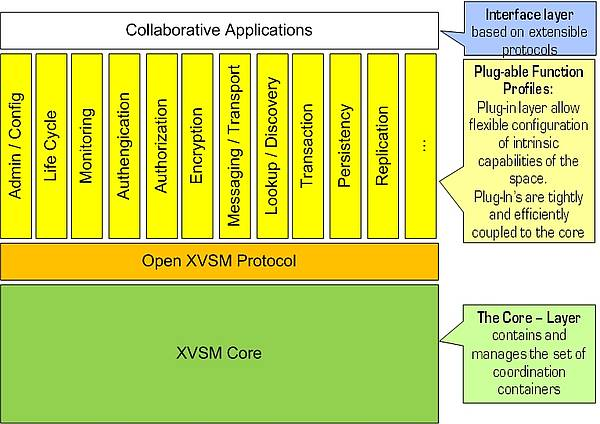
\includegraphics[width=0.7\linewidth]{./08570620af}
			\caption{}
			\label{fig:08570620af}
		\end{figure}
	

			\lbrack Quelle:http://www.complang.tuwien.ac.at/eva/SBC-Group/sbcGroupIndex.html \rbrack \\ \\ \\
		Unterschied zum Linda(JavaSpaces)Ansatz ist, dass die Daten in Container gespeichert werden und nicht direkt in den Space und die Daten mit Einträgen, Koordinaten und Containern leichter gefunden werden können.
		XVSM integriert das Konzept von Peer-2-Peer Netzwerken um ein Verteiltes Geteilten Space zu erzeugen.
		
		\subsection{Implementierungen}
			\begin{itemize}
				\item MozardSpaces
				\item XcoSpaces
				\item TinySpaces
			\end{itemize}
		
		
		\section{TinySpaces}
			Tinyspaces setzt auf das XVSM Prinzip auf und benutzt das .Net Framework. Da es bei dem XVSM Prinzip noch nicht vollkommen mit allen Implementierungen kompatibel war(z.B für embeded devices nicht perfomant genug) erschuf man Tinyspaces. 
			TinySpaces soll es erleichtern mit SBC zu arbeiten, da es unnötige schichten entfernt. 
			TinySpaces nutzt die Unterstützung von Contracts die sagen wie man ein bestimmtes Interface ansprechen soll.
			Durch die Nutzung von Contracts ist es möglich die Komponenten zu ändern/ersetzen und der Benutzer muss nur denn Contract kennen um zu wissen wie er mit der Komponente interagieren muss. Da man bei der Programmierung der Applikation darauf zielen sollte das alle Komponenten auf denn Contract aufbauen sollten.\\
		
		\section{GSpaces}
		Geht von dem selben Ansatz aus wie JavaSpaces(Tuple Spaces) hat aber einen großen Unterschied. GSpaces hat zwar Tupel, benutzt diese aber mit Replikationsrichtlinien.  Bei einem Aufruf wird ein lokaler Aufrufverarbeiter aufgerufen und es wird nachgeschaut welche Operation ausgeführt werden muss. Bei  einem Aufruf wird erst mal nachgeschaut welche Richtlinien angewendet werden müssen. Nachdem man die Auswahl getroffen hat wird die Anfrage weiter an einen Verteilungsmanager geleitet.  Wenn dann zB gelesen werden soll und es auf Master-Slave-Richtlinie basiert wird einfach die read Operation auf dem lokalem Datensatz(Slice) gelesen. Falls es aber eine write Operation ist muss der Verteilungsmanager beim Master Server anfragen ob er schreiben darf und dann kann er erst weiter schreiben.	
	
\chapter{Quellen}
	Primärquellen:\\
	\lbrack 14\rbrack Verteilete Systeme Prinzipien und Paradigmen, A. Tannenbaum, 2. Auflage \\
	\lbrack 15\rbrack Peer-toPeer Systems and Applications 2005, R. Steinmetz,K. Wehrle\\
	\lbrack 16\rbrack http://www.spacebasedcomputing.org/, Aufgerufen am 13.12.2013\\
	
	Sekundärquellen:\\
	\lbrack 1\rbrack http://www.nik.no/2002/Engelhardtsen.pdf \\
	\lbrack 2\rbrack Diplomarbeit,Integration von Corso Space-Based Computing in J2EE,Johannes Marchart\\
	\lbrack 3\rbrack Diplomarbeit,Design and Implementation of JavaSpaces API Standart for XSVM, Laszlo Keszthelyi\\
	\lbrack 4\rbrack http://wiki.gigaspaces.com/wiki/display/XAP9/Terminology+-+Space-Based+Architecture\\
	\lbrack 5\rbrack http://www.slideshare.net/amin59/an-introduction-to-space-based-architecture\\
	\lbrack 6\rbrack http://www.gigaspaces.com/WhitePapers\#a1 \\
	\lbrack 7\rbrack Diplomarbeit, Design and Implementation of TinySpaces, Alexander Marek \\
	\lbrack 8\rbrack http://www.spacebasedcomputing.org/fileadmin/files/SBC-Paradigm-v1.0.pdf \\
	\lbrack 9\rbrack http://elib.uni-stuttgart.de/opus/volltexte/2006/2580/pdf/TR\_2006\_05.pdf \\
	\lbrack 10\rbrack http://www.wsmo.org/TR/d21/v0.1/20050613/d21.v01.pdf \\
	\lbrack 11\rbrack http://www.mozartspaces.org/2.2-SNAPSHOT/docs/MozartSpaces\_DA\_Martin-Barisits.pdf \\
	\lbrack 12\rbrack Dissertation, Managing Complex and Dynamic Software Systems with Space-Based Computing, Richard Mordinyi \\
	\lbrack 13\rbrack Peer-to-Peer Systems III 2005, G. Voelker, S Shenker \\
	

\end{document}